\documentclass[11pt,a4paper]{article}
\usepackage{ConfigMP}
\usepackage{graphicx}
\usepackage{url}
\usepackage{float} % permite [H]: figuras en línea con el texto, sin flotar

% ================================
% INFORMACIÓN DEL DOCUMENTO
% ================================

% Información del miniproyecto
\newcommand{\claveproyecto}{MP-26-070}
\newcommand{\tituloproyecto}{Desarrollo asistido por Inteligencia Artificial de un resolvedor de sistemas de ecuaciones complejas para análisis de circuitos}
\newcommand{\autores}{Iker Emiliano Barrera García, Orlando Contreras Reyes }
\newcommand{\adscripciones}{Departamento de Sistemas Eletrónicos, Centro de Ciencias Básicas, Universidad Autónoma de Aguascalientes}

\begin{document}

% ================================
% TÍTULO Y INFORMACIÓN DEL PROYECTO
% ================================
\doctitle{MINIPROYECTOS 2026}{\tituloproyecto}{}

\projectdata{\claveproyecto}{\tituloproyecto}{\autores}{\adscripciones}

% ================================
% INTRODUCCIÓN
% ================================
\section{Introduccion}

El análisis de circuitos es una de las tareas más importantes del ingeniero, pues aplica conceptos matemáticos y físicos para obtener parámetros como voltaje o corriente, siendo la base de gran parte de la tecnología actual. Sin embargo, resolver de forma eficiente los sistemas de ecuaciones complejas que surgen en el análisis de CA rara vez cuenta con herramientas prácticas y portátiles dentro del aula. Las soluciones habituales han sido comprar una calculadora especializada, usar simuladores de calculadora en el celular (como Droid48, que emula la HP-48G)  o aplicar manualmente la regla de Cramer.

Estas soluciones presentan limitaciones claras: la regla de Cramer es poco eficiente; las calculadoras físicas y simuladas tienen un ingreso de datos tedioso y muestran resultados solo en forma rectangular o polar, nunca ambas y su uso indiscriminado puede derivar en deshonestidad académica cuando se recurre a la IA o a terceros sin comprender el proceso.

Ante esto, un equipo de estudiantes desarrolló una aplicación de escritorio, empaquetada como ejecutable (.exe), como primer prototipo hacia futuras versiones en Android y hardware dedicado. Cabe destacar que este prototipo fue diseñado en conjunto con IA, lo que demuestra el alcance de un ingeniero electrónico apoyado en estas herramientas.
\newpage
% ================================
% OBJETIVOS
% ================================
\section{Objetivos}

\subsection*{Objetivo General}
Desarrollar, con apoyo de herramientas de inteligencia artificial, una calculadora de escritorio capaz de resolver sistemas de ecuaciones con números complejos aplicados al análisis de circuitos de CA (mallas y nodos), mediante álgebra lineal numérica, con interfaz gráfica y distribución como ejecutable independiente para Windows y GNU/Linux.

\subsection*{Objetivos Específicos}
\begin{itemize}
    \item Implementar el ingreso de datos complejos en forma rectangular ($a+jb$) y polar ($r\angle\theta^\circ$).
    \item Resolver sistemas de $n \times n$ con coeficientes complejos mediante \texttt{numpy.linalg.solve}, evitando la regla de Cramer manual.
    \item Diseñar una interfaz con CustomTkinter que muestre resultados en ambas representaciones simultáneamente.
    \item Empaquetar la aplicación como ejecutable autónomo mediante PyInstaller.
    \item Validar la herramienta contra ejercicios de análisis de circuitos resueltos manualmente.
\end{itemize}

% ================================
% MATERIALES Y MÉTODOS
% ================================
\section{Materiales y metodos}

El desarrollo se dividió en tres fases: selección de herramientas y arquitectura, implementación de los algoritmos con apoyo de IA, y construcción de la interfaz gráfica con su empaquetado.

\subsection*{Materiales y Herramientas}
\begin{itemize}
    \item \textbf{Entorno y lenguaje:} Visual Studio Code v1.85+, Python 3.10+.
    \item \textbf{Librerías:} \texttt{NumPy} (resolución de sistemas complejos), \texttt{CustomTkinter}/\texttt{Tkinter} (GUI), \texttt{Pillow} (recursos gráficos), \texttt{OS}/\texttt{JSON} (persistencia e historiales).
    \item \textbf{IA:} Asistente de código ChatGPT (OpenAI), usado para optimizar fragmentos, refactorizar y agilizar el diseño de la GUI.
    \item \textbf{Compilación:} \texttt{PyInstaller}, para generar el ejecutable autónomo.
\end{itemize}

\begin{figure}[H]
    \centering
    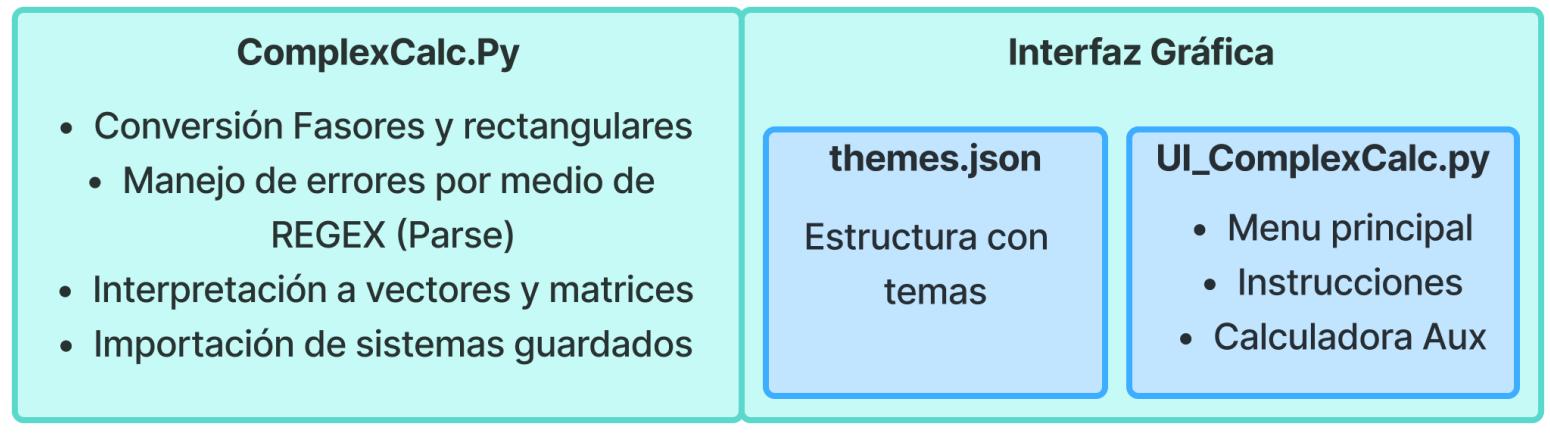
\includegraphics[width=0.85\linewidth]{../../src/Architecture.png}
    \caption{Arquitectura}
    \label{fig:arquitectura}
\end{figure}
\newpage
\subsection*{Arquitectura y Algoritmos}
Un sistema de mallas o nodos de $n \times n$ se representa matricialmente como:

\begin{equation}
    [\mathbf{Z}] [\mathbf{I}] = [\mathbf{V}] \quad \rightarrow \quad [\mathbf{I}] = [\mathbf{Z}]^{-1} [\mathbf{V}]
\end{equation}

donde $[\mathbf{Z}]$ es la matriz de impedancias complejas, $[\mathbf{I}]$ el vector de corrientes desconocidas y $[\mathbf{V}]$ el vector de fuentes. La resolución se realiza con el solver de \texttt{NumPy}, garantizando precisión y eficiencia frente a la regla de Cramer. Una vez calculado el vector solución, cada componente se convierte automáticamente a forma polar ($r = \sqrt{a^2 + b^2}, \; \theta = \arctan(b/a)$) para mostrar ambos formatos al usuario.

\subsection*{Flujo de Trabajo con IA}
El desarrollo integró un ciclo iterativo con ChatGPT: generación de maquetas iniciales (ventanas, contenedores, celdas matriciales editables), resolución de errores al manipular arreglos complejos en tiempo real, refactorización para separar cálculo y renderizado, y supervisión/validación humana de cada segmento generado, probado contra ejercicios teóricos.

\subsection*{Interfaz y Empaquetado}
Se adoptó \texttt{CustomTkinter} con un archivo \texttt{.json} de estilos, agregando una barra de herramientas para guardar matrices, limpiar celdas y alternar el formato de salida. El programa se compiló con \texttt{PyInstaller} (\texttt{--onefile --noconsole}), empaquetando intérprete, dependencias y recursos en un solo ejecutable.

\subsection*{Filosofía}
El proyecto se guió por las filosofías \textit{Open Source} y \textit{Vibe Coding}: con solo bases de C para microcontroladores, los autores construyeron una herramienta funcional apoyándose en IA, demostrando que unas buenas bases de programación bastan para desarrollar soluciones prácticas. Se optó por Python por agilizar la implementación sin sacrificar funcionalidad. 
\bigskip
\noindent \textit{\textbf{Aclaración de autoría y licenciamiento:} Parte de las estructuras de código fuente e interfaz fueron desarrolladas con apoyo del modelo de inteligencia artificial ChatGPT.}

% ================================
% RESULTADOS Y DISCUSIONES
% ================================
\section{Resultados y discusiones}

La calculadora facilita la resolución de sistemas lineales reales y complejos, siendo útil en cursos como Análisis de Circuitos, Electrónica, Señales y Sistemas y Métodos Matemáticos, donde el manejo de cantidades fasoriales es fundamental. Cuenta con historial de operaciones y, al ser gratuita y multiplataforma, resulta una alternativa accesible en el ámbito académico.

En la Figura~\ref{fig:interfaz2} se muestra la solución de un sistema y la interfaz de la calculadora.

\begin{figure}[!h]
    \centering
    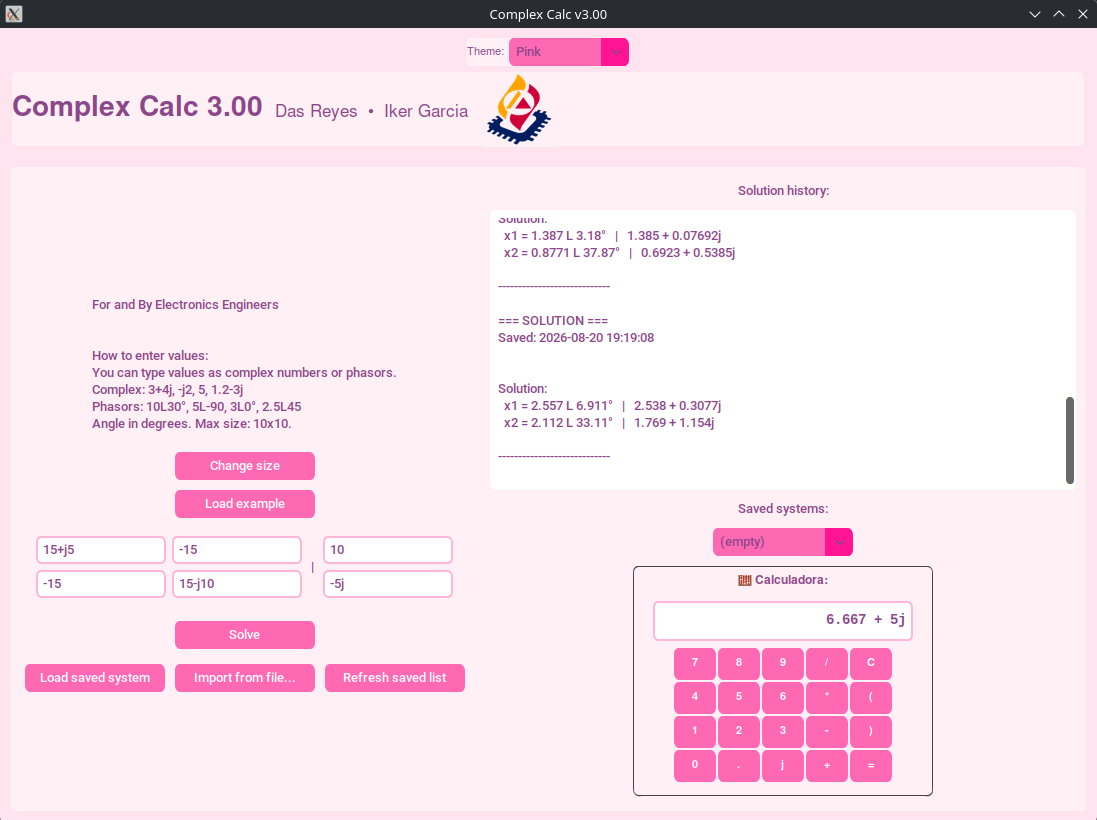
\includegraphics[width=0.55\linewidth]{../../src/RectSol.png}
    \caption{Solución de un sistema complejo.}
    \label{fig:interfaz2}
\end{figure}

Durante el desarrollo surgieron tres retos principales: lograr una interfaz intuitiva para usuarios sin experiencia, corregir errores en el guardado y carga de matrices, y personalizar visualmente Tkinter modificando el archivo \texttt{.json} de estilos.

% ================================
% CONCLUSIONES
% ================================
\section{Conclusiones}

El proyecto comprobó que la inteligencia artificial es útil en programación cuando se usa como apoyo y no como sustituto del conocimiento del programador: partiendo solo de bases de C para microcontroladores, fue posible construir y validar una aplicación funcional para resolver sistemas de ecuaciones complejas aplicados al análisis de circuitos. Se obtuvo una herramienta que convierte números complejos entre forma rectangular y polar mediante NumPy, distribuida como ejecutable autónomo sin necesidad de configurar un entorno de programación.

% ================================
% REFERENCIAS
% ================================
\section{Referencias}

[1] Anton, H., Rorres, C. (2013). \textit{Álgebra lineal con aplicaciones}. Wiley.

[2] Lay, D. C. (2012). \textit{Álgebra lineal y sus aplicaciones}. 4.\textsuperscript{a} ed., Pearson.

[3] NumPy Developers. (2026). \textit{numpy.linalg.solve — NumPy v2.5 Manual}. \url{https://numpy.org/doc/stable/reference/generated/numpy.linalg.solve.html}

[4] Python Software Foundation. (2026). \textit{tkinter — Python interface to Tcl/Tk}. \url{https://docs.python.org/3/library/tkinter.html}

[5] Cortesi, D., Bajo, G., McMillan, W. (2026). \textit{PyInstaller Manual}. \url{https://pyinstaller.org/en/stable/}

[6] OpenAI. (2026). \textit{ChatGPT}. \url{https://chatgpt.com/}

\end{document}